		\tikzsetfigurename{Fig_module_2_1_13_Arctangent_Arccotangent}

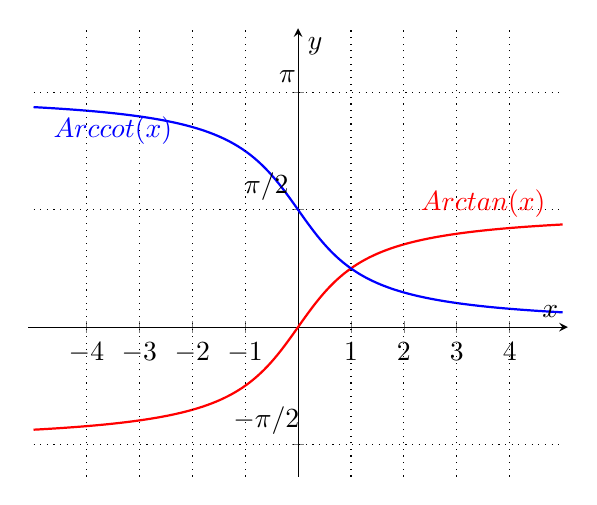
\begin{tikzpicture}
\begin{axis}[ylabel=$y$,xlabel=$x$,
axis lines=middle,
xmin=-5.1,xmax = 5.1,ymin=-2,ymax=4,
%minor x tick num = 0.5,
xtick={-4,-3,-2,-1,0,1,2,3,4},
domain=-5:5,
xticklabel={},
ytick={-pi,-pi/2,0,pi/2,pi}, 
yticklabel={\textcolor{white}\ticknum}
]
\addplot[samples=500,color=red,thick] {rad(atan(x))};
\addplot[samples=500,color=blue,thick] {rad(90-atan(x))};



\draw[dotted] (-4,-2)--(-4,4);
\draw[dotted] (-3,-2)--(-3,4);
\draw[dotted] (-2,-2)--(-2,4);
\draw[dotted] (-1,-2)--(-1,4);

\draw[dotted] (1,-2)--(1,4);
\draw[dotted] (2,-2)--(2,4);
\draw[dotted] (3,-2)--(3,4);
\draw[dotted] (4,-2)--(4,4);



\draw[dotted] (-5,-pi/2)--(5,-pi/2);
\draw[dotted] (-5,pi/2)--(5,pi/2);
\draw[dotted] (-5,pi)--(5,pi);


\draw[](-0.6,-pi/2) node[left,above]{$-\pi/2$}; 
\draw[](-0.6,pi/2) node[left,above]{$\pi/2$}; 
\draw[](-0.2,pi) node[left,above]{$\pi$}; 

\draw[](-3.5,pi-0.2) node[left,below,blue]{$\text{Arccot}(x)$}; 
\draw[](3.5,pi/2+0.4) node[left,below,red]{$\text{Arctan}(x)$}; 


\end{axis}
\end{tikzpicture}